% labels:
% cap:introducao
% sec:motivacao_proposta
% sec:tools
% sec:asteroids
% sec:gymretro
% sec:tensorflow
% sec:proposta

%% ---------------------------------------------------------------------------- %
\chapter{Introdução}
\label{cap:introducao}
%% ---------------------------------------------------------------------------- %

Inteligência artificial, ou IA, é uma área de estudos que pode ser definida de diversas formas, como construir uma máquina que realize com sucesso tarefas tradicionalmente feitas por humanos, ou que aja como um humano.
Envolvendo filosofia, matemática, economia, neurociência, psicologia, computação e até mesmo linguística ao longo de sua história, ela abrangeu e ainda abrange diversos campos da ciência, com profissionais de várias formações diferentes podendo contribuir para seus avanços.
Existem inúmeros desafios atualmente: alguns resolvidos, como vencer de jogadores profissionais de Xadrez, mas muitos ainda sendo abordados, podendo ser uma busca por alguma solução, ou por uma solução mais eficiente que a já existente.

%Um tipo muito conhecido de inteligência artificial dos dias atuais é a que controla oponentes em jogos eletrônicos.
%Porém, nesses casos, os adversários apenas seguem um conjunto pré-determinado de regras escritas pelo desenvolvedor, não possuindo a capacidade de se adaptar como seres humanos fazem.
%Por mais que isso seja um tipo de IA e que possa ser mais eficiente em determinadas tarefas, não se assemelha à forma que as pessoas pensam e jogam.
É interessante a forma como, em particular, seres humanos aprendem.
Crianças pequenas e bebês principalmente aprendem interagindo com o ambiente: tocam nos objetos, tentam entender aquilo que os rodeia e qual o resultado de suas ações, mesmo que inconscientemente.
%Em um jogo, se não passar por um tutorial ou ler um manual, não será muito diferente: o jogador precisará descobrir o que é hostíl, o que cada comando faz e qual o objetivo.
Avanços recentes em inteligência artificial permitiram que máquinas simulem esse tipo de aprendizado por meio de \textbf{aprendizado por reforço}.
Entretanto, para muitos casos, só essa técnica não é o suficiente.
Utilizando jogos como exemplo, uma pessoa consegue inferir o que é inimigo e o que é terreno quando aparece na tela do jogo em poucos movimentos ou até já supor a partir de experiências passadas com jogos diferentes.
Para um computador, um pixel que mude de posição já faz ele não conseguir mais distinguir o que está vendo, tendo que re-aprender a cada nova combinação de pixels detectada.
Em outras palavras, seres humanos conseguem abstrair as informações que enxergam com facilidade, enquanto os computadores não.

Se computadores não conseguem mais identificar um objeto na tela por causa de um pixel que esteja diferente, como sistemas de detecção de imagem funcionam?
%Essa é uma questão que avanços recentes em visão computacional, campo interdisciplinar que estuda a capacidade dos computadores de enxergarem imagens e vídeos, ajudou a resolver.
Utilizando uma variante de rede neural profunda (\textit{deep neural network}) chamada \textbf{rede neural convolucional} (\textit{convolutional neural network} (CNN)), é possível fazer uma inteligência artificial abstrair essas informações e inferir que um objeto em diferentes lugares da tela, assumindo diferentes tamanhos, são o mesmo.

%% ---------------------------------------------------------------------------- %
\section{Motivação e Proposta}
\label{sec:motivacao_proposta}

A proposta deste trabalho surgiu do interesse por uma técnica de aprendizado de máquina não estudada nas disciplinas de inteligência artificial do curso.
%Unindo o antigo interesse por jogos com o recente por inteligência artificial, surgiu a proposta deste trabalho de conclusão de curso.
Aplicando os conhecimentos adquiridos na faculdade, o objetivo deste trabalho é fazer um estudo de caso de \textit{deep Q-learning} aplicado a ambientes com características distintas.
%O estudo será feito em três domínios com características distintas: o \textit{Gridworld}, o \textit{Pong} e o \textit{Asteroids}.
%principal objetivo é criar uma inteligência artificial que aprenda a jogar o jogo eletrônico \textit{Asteroids}.

As ferramentas utilizadas, descritas na próxima seção, foram o Gym e Gym-Retro como interface, o Stella como emulador e a API do TensorFlow para a computação.
As técnicas de aprendizado de máquina aplicadas, descritas no capítulo seguinte, foram \textbf{aprendizado por reforço} e \textbf{rede neural convolucional}, mais especificamente a união das duas, conhecida como \textit{\textbf{deep reinforcement learning}} ou \textit{\textbf{deep Q-learning}}~\cite{DBLP:journals/corr/MnihKSGAWR13}.

Espera-se conseguir construir arquiteturas de \textit{deep Q-learning} pela qual o agente consiga montar um modelo que tenha sucesso no respectivo ambiente.
%Espera-se conseguir construir uma arquitetura de aprendizado que permita a inteligência artificial desenvolver um modelo capaz de jogar com um desempenho pelo menos próximo de um ser humano.
%Em caso negativo, tentar explicar o motivo de o computador ter um desempenho notavelmente pior.

\section{Ferramentas}
\label{sec:tools}
Nesta seção, serão apresentados os ambientes e as principais ferramentas utilizadas no desenvolvimento deste trabalho, uma breve descrição sobre elas e o motivo de suas escolhas.

\subsection{\textit{Gridworld}}
\label{sec:gridworld}

\textit{Gridworld} é um exemplo clássico em estudos e ensinamentos de aprendizado por reforço.
Ele consiste em um mapa de espaços quadrados em que o agente começa em um deles e pode se mover para cima, direita, esquerda ou baixo, contanto que o espaço seja válido.
Alguns dos espaços geram recompensa positiva (objetivo) e outros geram recompensa negativa (armadilha) ao ser alcançado, além de encerrarem o episódio e fazerem o agente retornar ao ponto inicial.
O desenvolvedor pode optar por gerar pequenas recompensas positivas ou negativas a cada passo, mesmo que não alcance um estado terminal, para analisar seu comportamente em tais circunstâncias.

\begin{figure}[h!]
  \begin{minipage}[b]{.6\textwidth}
  \centering
  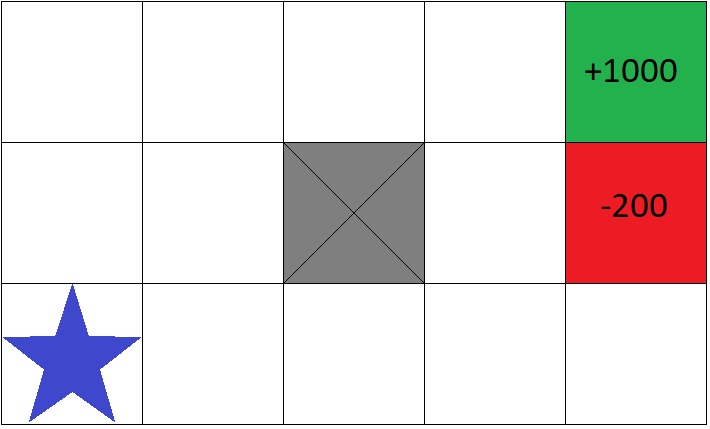
\includegraphics[scale=.35]{gridworld_example01}
  %\caption{Exemplo de tela do jogo. O números no topo da tela são pontuação e quantidade de vidas respectivamente. A nave, no centro, está atirando. Asteróides espalhados pela tela.}
  \end{minipage}
  \hfill
  \begin{minipage}[b]{.35\textwidth}
  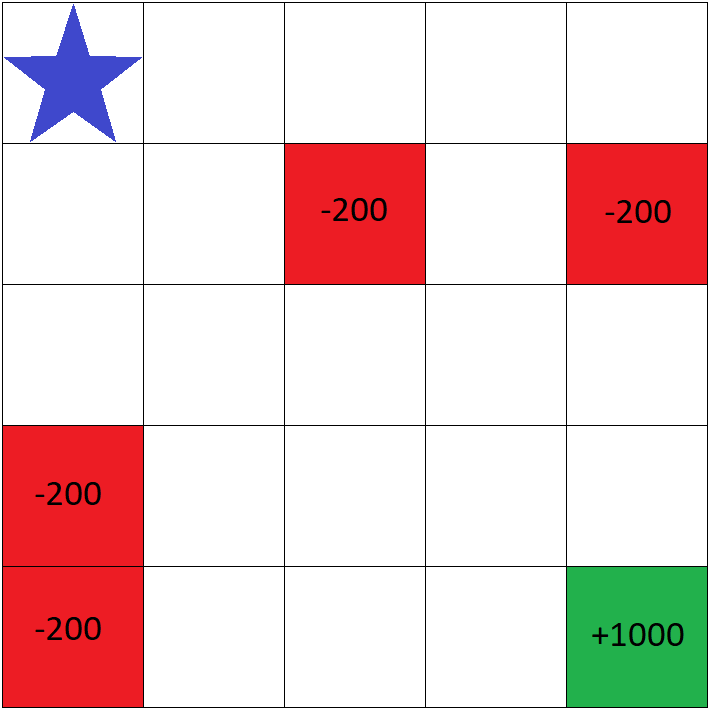
\includegraphics[scale=.2105]{gridworld_example02}
  %\caption{Exemplo de tela do jogo. A nave acaba de destruir um asteróide de menor tamanho e está recebendo uma recompensa de 100 pontos por isso. Asteróides podem ter diversas cores.}
  \end{minipage}
  \centering
  \caption{Exemplos de mapas de \textit{Gridworld}. A estrela azul indica a posição inicial do agente, o espaço cinza com um $\times$ indica um espaço inválido, o verde com +1000 representa o objetivo e os vermelhos com -200 representam as armadilhas.}
\end{figure}

O número de estados deste ambiente é igual ao número de espaços válidos, uma vez que são definidos pela posição em que o agente se encontra.

\textit{Gridworld} é o ambiente mais simples estudado neste trabalho.

\subsection{\textit{Pong} - Atari2600}
\label{sec:pong}

\textit{Pong} foi um dos primeiros jogos criados e o primeiro desenvolvido pela Atari, lançado em novembro de 1972.
O jogo simula uma partida de tênis de mesa por meio de duas barras verticais, uma do lado esquerdo e uma do lado direito, e uma bola que se move pela tela.
Cada jogador controla uma das barras movendo-a para cima e para baixo, rebatendo a bola para evitar que chegue no fim da tela do próprio lado enquanto tenta fazê-la chegar no fim da tela do lado do adversário.
A principal diferença entre as versões do jogo é o número de pontos necessários para vencer.

A versão do \textit{Pong} utilizada neste trabalho é a do Atari2600, emulada pelo emulador Stella.
Nesta iteração, vence o jogador que fizer 21 pontos primeiro.

\begin{figure}[h!]
  \begin{minipage}[b]{.5\textwidth}
  \centering
  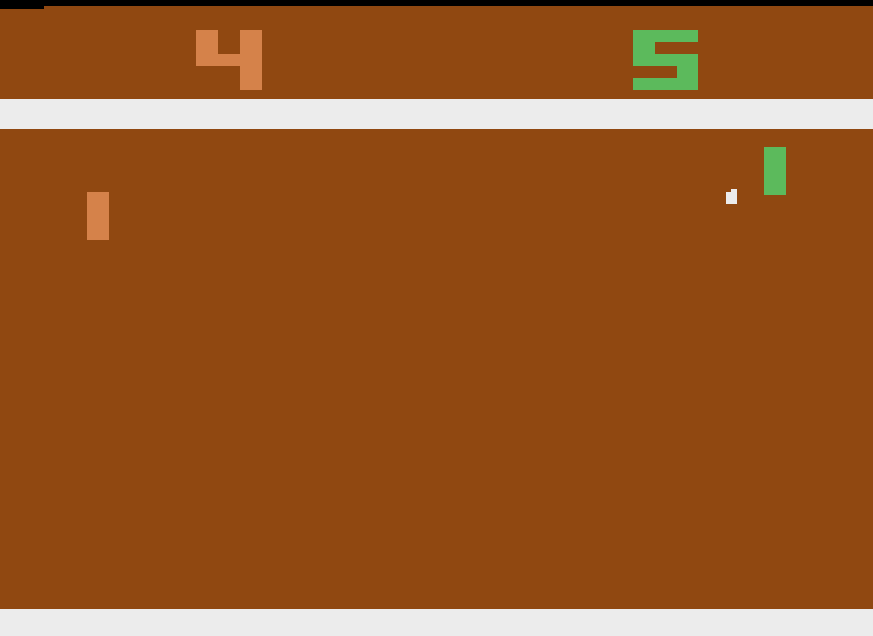
\includegraphics[scale=.25]{pong_example01}
  %\caption{Exemplo de tela do jogo. O números no topo da tela são pontuação e quantidade de vidas respectivamente. A nave, no centro, está atirando. Asteróides espalhados pela tela.}
  \end{minipage}
  \hfill
  \begin{minipage}[b]{.5\textwidth}
  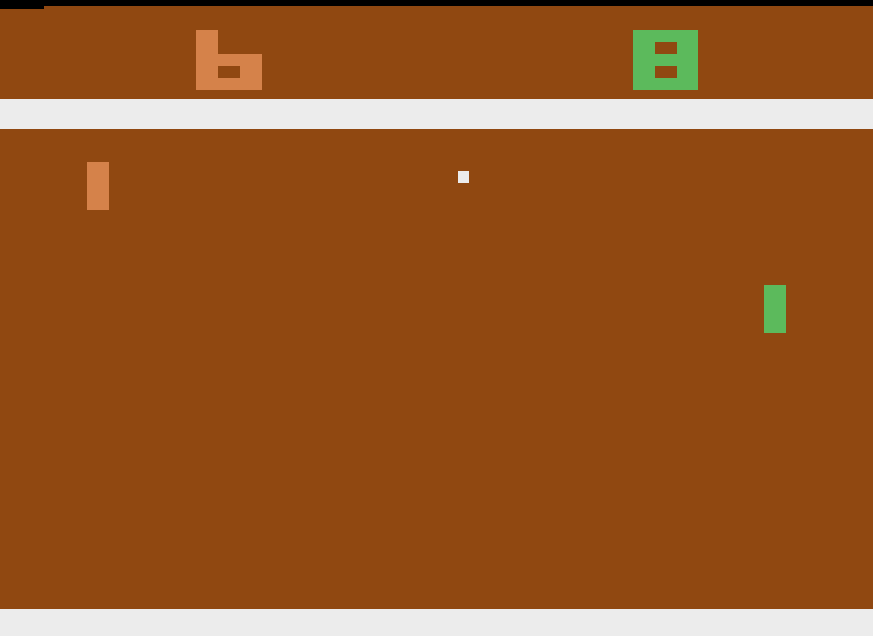
\includegraphics[scale=.25]{pong_example02}
  %\caption{Exemplo de tela do jogo. A nave acaba de destruir um asteróide de menor tamanho e está recebendo uma recompensa de 100 pontos por isso. Asteróides podem ter diversas cores.}
  \end{minipage}
  \caption{Exemplos de tela do jogo no emulador Stella. O jogador controla a barra verde, do lado direito da tela caso o oponente seja a IA escrita pelos desenvolvedores. O ponto branco no meio da tela é a bola, as barras brancas representam os limites superior e inferior do campo e os números no topo indicam a pontuação de cada jogador.}
\end{figure}

Os estados são definidos pela tela do jogo, que é uma matriz de 210x160 pixels, com cada pixel tendo 3 canais de cor.
Esses canais variam de 0 a 255 e a combinação de seus valores determinam a cor do pixel dentro de uma paleta de 128 cores.

\textit{Pong} é o ambiente de complexidade média estudada neste trabalho.

\subsection{\textit{Asteroids} - Atari2600}
\label{sec:asteroids}

\textit{Asteroids} é um jogo de fliperama
%do gênero \textit{top down shooter} (jogo eletrônico de tiro visto de cima)
 lançado em novembro de 1979 pela
 %então desenvolvedora de jogos eletrônicos Atari Inc, atualmente conhecida como
 Atari.
O jogador controla uma nave espacial em um campo de asteróides, tentando destruí-los enquanto tenta sobreviver.
Quando um asteróide é destruído, outros menores aparecem no lugar.
As principais diferenças entre as iterações de \textit{Asteroids} incluem a presença de naves espaciais inimigas que atiram contra o jogador, formatos e tamanhos diferentes dos asteróides e direção que eles se movem.

A versão de \textit{Asteroids} utilizada neste trabalho é a do Atari2600, emulada pelo emulador Stella.
Nesta iteração, não existem naves espaciais inimigas, apenas asteróides que assumem três tamanhos distintos, começando sempre pelo maior, que vale menos pontos enquanto o menor vale mais.
%, sendo o maior deles o inicial, e três formatos diferentes, mas de aproximadamente mesma altura e largura, e cores diferentes.
%Destruir um asteróide faz outros menores aparecerem no lugar e dão pontos para o jogador, com o maior valendo menos e o menor valendo mais.
%Quando um asteróide grande (tamanho inicial) é destruído, outros dois de tamanho médio aparecem no lugar; após um asteróide de tamanho médio ser destruído, um de tamanho pequeno aparece em seu lugar.
%Destruir um asteróide grande gera uma recompensa de 20 pontos, destruir um médio gera uma recompensa de 50, e um pequeno gera uma de 100 pontos.
A principal forma de destruir um asteróide e ganhar pontos é atirando neles.
%, mas isso também ocorre quando há colisão entre a nave e um alvo.
%Isso reduz a quantidade de vidas disponíveis e, portanto, não é um método recomendado, dado que diminui a quantidade total de pontos ganha no final do jogo.
%Os asteróides também têm uma velocidade horizontal e vertical fixa para cada um.
%A cada \textit{frame}, se movem 1 pixel na vertical e a cada aproximadamente 12 frames se movem um 1 pixel na horizontal, resultando em seus movimentos serem principalmente verticais.
O jogador possui quatro vidas inicialmente e cinco ações para jogar: mover-se para frente, girar a nave no sentido horário, girar a nave no sentido anti-horário, mover-se no hiper-espaço, e atirar para frente.
Mover-se para frente e girar são as principais formas de movimento no jogo, enquanto atirar é a de destruir asteróides e ganhar pontos.
Mover-se no hiper-espaço consiste em fazer a nave desaparecer por alguns instantes e reaparecer em um local aleatório da tela.

\begin{figure}[h!]
  \begin{minipage}[b]{.5\textwidth}
  \centering
  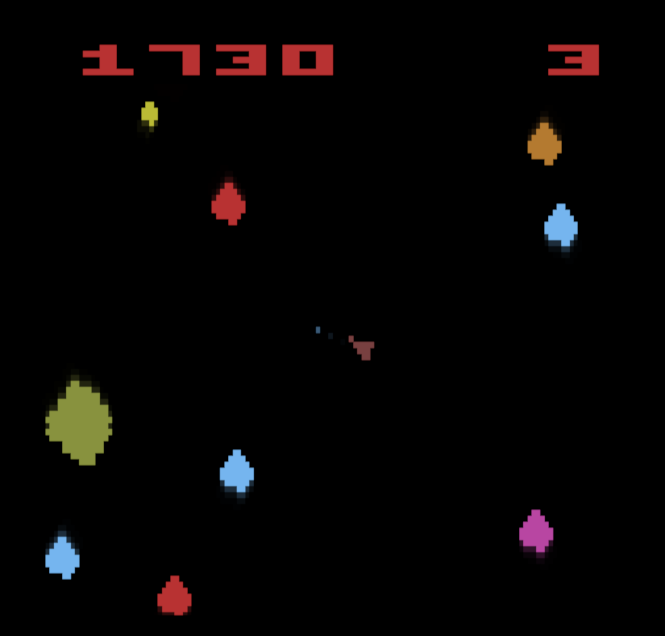
\includegraphics[scale=1.41]{asteroids_example01}
  %\caption{Exemplo de tela do jogo. O números no topo da tela são pontuação e quantidade de vidas respectivamente. A nave, no centro, está atirando. Asteróides espalhados pela tela.}
  \end{minipage}
  \hfill
  \begin{minipage}[b]{.5\textwidth}
  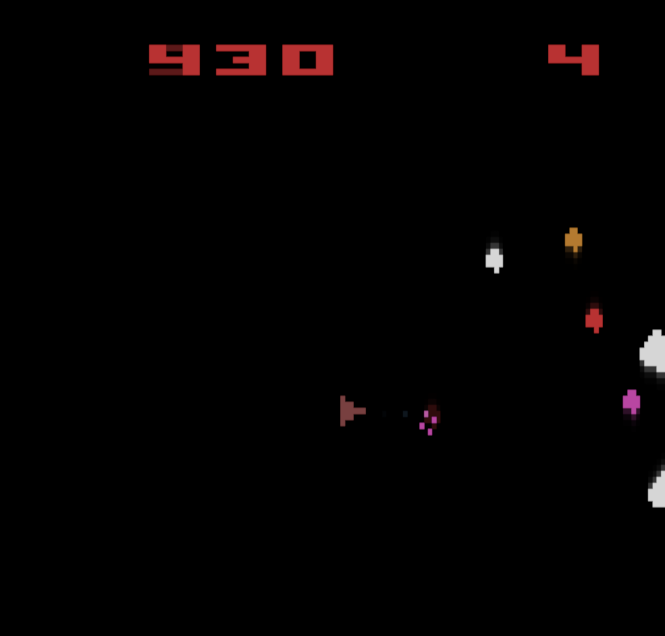
\includegraphics[scale=1.41]{asteroids_example02}
  %\caption{Exemplo de tela do jogo. A nave acaba de destruir um asteróide de menor tamanho e está recebendo uma recompensa de 100 pontos por isso. Asteróides podem ter diversas cores.}
  \end{minipage}
  \caption{Exemplos de tela do jogo no emulador Stella. O número no canto superior esquerdo é a pontuação e o do canto superior direito é a quantidade de vida restante que o jogador tem. A nave é o triângulo no meio da tela, o ponto azul próximo dela na imagem da esquerda é um tiro e o restante é asteróide. Na tela da direita, um asteróide acaba de ser destruído.}
\end{figure}

Assim como no \textit{Pong}, os estados são compostos por uma matriz de 210x160 pixels, cada um tendo 3 canais que determinam a cor.

\textit{Asteroids} é o mais complexo dos ambientes estudados neste trabalho.
%, podendo ser inclusive em cima de asteróides.
%Portanto, é um movimento arriscado, mas útil para fugir de situações complicadas.
%O jogador tem quatro vidas inicialmente.

%A tela do jogo é uma matriz de tamanho 210x160 pixels com cada pixel tendo três números, que variam de 0 a 255 cada, e que determinam sua cor de acordo com a escala RGB, tendo acesso a uma paleta de 128 cores (é necessário que esses três números atinjam um certo valor para mudar a cor do pixel).
%No topo da tela, há dois números indicando a pontuação total até o momento e quantidade de vidas restantes.
%Desconsiderando a moldura da tela, o espaço em que o jogo ocorre é de 177x152 pixels.

%\textit{Asteroids} é considerado um dos primeiros grandes sucessos da era de ouro dos jogos de fliperama, época em que os jogos eletrônicos começaram a se tornar comuns na cultura popular. 

%------------------------%

\subsection{Gym \& Gym-Retro}
\label{sec:gymretro}

Gym é uma plataforma para pesquisa de aprendizado por reforço desenvolvida e mantida pela empresa de pesquisas em inteligência artificial OpenAI.
Esta ferramenta auxilia na emulação de diversos ambientes diferentes, incluindo alguns poucos jogos de Atari (\textit{Pong} incluso, mas \textit{Asteroids} não) e ambientes 3D.
Utilizou-se o \textit{Frozen Lake}, removendo a aleatoriedade dos movimentos e criando um mapa personalizado do tamanho desejado, e o \textit{Pong} do Gym neste trabalho.

Gym-Retro é uma variante da Gym com ênfase em jogos eletrônicos antigos, como dos consoles Sega Genesis, Nintendo Entertainment System e Atari2600.
%Gym-Retro é uma plataforma para pesquisa de aprendizado por reforços e generalização em jogos desenvolvida e mantida pela empresa de pesquisas em inteligência artificial OpenAI.
%Essa ferramenta auxilia na emulação de diversos consoles de jogos eletrônicos, como Sega Genesis, Nintendo Entertainment System (NES) e Atari2600.
Para qualquer jogo que o usuário deseje emular, é necessário que ele tenha a ROM (\textit{Read Only Memory}) do jogo.
Utilizou-se o \textit{Asteroids} do Gym-Retro neste trabalho.

O principal motivo de estas ferramentas terem sido escolhidas é por permitirem emular o \textit{Pong} e o \textit{Asteroids}, além de possuir um ambiente semelhante ao \textit{Gridworld}.
%------------------------%
\subsection{TensorFlow}
\label{sec:tensorflow}

TensorFlow é um arcabouço de código aberto para computações numéricas de alta performance, desenvolvido e mantido pela Google.
Seu núcleo de computação numérica flexível permite o uso da biblioteca em diversos campos cienctíficos.
Oferece, em particular, grande suporte a aprendizado de máquina e aprendizado profundo, ou, como é mais conhecido, \textit{deep learning}.
Esta ferramenta foi escolhida por oferecer uma API em Python estável, ter grande suporte, comunidade ativa, e ser de código aberto.

%------------------------%

\section{Proposta}
\label{sec:proposta}

A proposta deste trabalho é fazer um estudo de caso da técnica \textit{deep Q-learning} em três ambientes digitais diferentes e ver o grau de sucesso obtido em cada um, utilizando como entrada apenas a tela do jogo (considerando o mapa do \textit{Gridworld} com o agente inserido como uma tela).
Gym e Gym-Retro servirão de interface enquanto o Stella emulará o jogo.
As técnicas de aprendizado de máquina utilizadas serão \textbf{aprendizado por reforço} e \textbf{rede neural convolucional}, em particular o \textbf{\textit{deep Q-learning}}, que é a junção dessas duas.

%A proposta do trabalho é criar uma arquitetura para que uma inteligência artificial seja capaz de aprender a jogar \textit{Asteroids} do Atari2600 tendo como entrada de dados apenas a tela do jogo, representada por uma matriz de pixels de 210x160 e 3 canais de cores.
%O emulador Stella e o Gym-Retro serão utilizados para emular o jogo e servir de interface com o jogo respectivamente.
